
\documentclass{article}

\usepackage{fullpage}
\usepackage{cite,enumerate}
\usepackage{color,graphics,graphicx}
\usepackage[cmex10]{amsmath}
\usepackage{amssymb,amsfonts,bm,amsthm}
\usepackage{booktabs}

\setcounter{secnumdepth}{2}
\DeclareMathOperator*{\minimize}{minimize}
\DeclareMathOperator*{\maximize}{maximize}
\DeclareMathOperator*{\subj}{subject\;to}
\newtheorem{definition}{Definition}

\newcommand{\commentGP}[1]{\noindent \textcolor{blue}{\emph{$<\,$GP: #1$\,>$}}}%
\newcommand{\commentGH}[1]{\noindent \textcolor{blue}{\emph{$<\,$GH: #1$\,>$}}}%
\newcommand{\commentWVL}[1]{\noindent \textcolor{blue}{\emph{$<\,$WVL: #1$\,>$}}}%

% Tikz
\usepackage{tikz}
\usepackage{pgfplots}
\pgfplotsset{compat=newest}
\usetikzlibrary{calc,positioning,shapes,matrix,patterns,decorations.pathmorphing}
\usetikzlibrary{decorations.markings,plotmarks}

% Define standardized height and width figures
\newlength\fheight
\setlength\fheight{4.5cm}
\newlength\fwidth
\setlength\fwidth{6cm}

% NOTATION
% General sets
\newcommand{\N}{\mathbb{N}}         % integer numbers
\newcommand{\R}{\mathbb{R}}         % real numbers
\newcommand{\C}{\mathbb{C}}         % complex numbers
\renewcommand{\S}{\mathbb{S}}       % symmetric matrices
\renewcommand{\H}{\mathbb{H}}       % Hermitian matrices
% General operators
\newcommand{\Tr}{\mathrm{Tr}}       % trace
% Selected superscripts
\renewcommand{\t}{\intercal}        % matrix transpose
\newcommand{\opt}{\star}                    % optimal points and values
\newcommand{\adj}{\ast}                     % adjoint operator
% Selected subscripts
\newcommand{\feas}{\mathrm{f}}              % feasible
\newcommand{\strfeas}{\mathrm{sf}}          % strictly feasible
% Parametric program
\newcommand{\ppar}{\theta}                          % parameter in the pprog
\newcommand{\Ppar}{{\bm{\theta}}}                   % set of parameters
\newcommand{\pPar}{\Theta}                          % matrix parameters
\newcommand{\PPar}{{\bm{\Theta}}}                   % set of matrix parameters
\newcommand{\X}{\mathbf{X}}                         % domain of primal variable x
\newcommand{\Y}{\mathbf{Y}}                         % domain of dual variable y
\newcommand{\K}{\mathbf{K}}                         % cone in \Y
\newcommand{\calF}{\mathcal{F}}                     % linear mapping defining the constraints
\newcommand{\Pfeas}{\Ppar^\Pi_\feas}                % set of parameters for which the primal is feasible
\newcommand{\Pstrfeas}{\Ppar^\Pi_\strfeas}          % set of parameters for which the primal is feasible
\newcommand{\Dfeas}{\Ppar^\Delta_\feas}             % set of parameters for which the dual is feasible
\newcommand{\Dstrfeas}{\Ppar^\Delta_\strfeas}       % set of parameters for which the dual is feasible
% Infinite dimensional reformulation
\newcommand{\Xm}{{\bm{\mathcal{X}}_{\Ppar}}}        % set of continuous functions \Ppar -> \X
\newcommand{\Ym}{{\bm{\mathcal{Y}}_{\Ppar}}}        % set of continuous functions \Ppar -> \Y
\newcommand{\Km}{{\bm{\mathcal{K}}}}                % cone in \Ym
% Approximation
\newcommand{\bx}{b^x}               % basis functions of \hat{x}
\newcommand{\bxa}{\bx_\alpha}       % \alpha'th basis functions of \hat{x}
\newcommand{\cx}{\textsf{x}}        % coefficients of \hat{x}   ??? should we use $c^x$ ???
\newcommand{\cxa}{\cx_\alpha}       % \alpha'th coefficient of \hat{x}
\newcommand{\nx}{{n_x}}             % number of basis functions of \hat{x}
\newcommand{\by}{b^y}               % basis functions of \hat{y}
\newcommand{\bya}{\by_\alpha}       % \alpha'th basis functions of \hat{y}
\newcommand{\cy}{\textsf{y}}        % coefficients of \hat{y}   ??? should we use $c^y$ ???
\newcommand{\cya}{\cy_\alpha}       % \alpha'th coefficient of \hat{y}
\newcommand{\ny}{{n_y}}             % number of basis functions of \hat{y}
\newcommand{\Alpha}{\bm{\alpha}}    % set of multi-indices
\newcommand{\meanh}{\bar{h}}        % averaged h
\newcommand{\meanha}{\meanh_\alpha} % \alpha'th entry of averaged h
\newcommand{\meang}{\bar{g}}        % averaged g
\newcommand{\meanga}{\meang_\alpha} % \alpha'th entry of averaged g
% B-spline approximation
\newcommand{\pparL}{\underline{\ppar}}
\newcommand{\pparU}{\overline{\ppar}}
\newcommand{\bPi}{b^\Pi}                % basis functions of constraints in \Pi
\newcommand{\bPia}{b^\Pi_\alpha}        % \alpha'th basis functions of constraints in \Pi
\newcommand{\nPi}{{n_\Pi}}              % number of basis functions of constraints in \Pi
\newcommand{\cg}{\textsf{g}}            % coefficients of g     ??? should we use $c^g$ ???
\newcommand{\cga}{\textsf{g}_\alpha}    % \alpha'th coefficients of g
\newcommand{\bDelta}{b^\Delta}          % basis functions of constraints in \Delta
\newcommand{\bDeltaa}{b^\Delta_\alpha}  % \alpha'th basis functions of constraints in \Delta
\newcommand{\nDelta}{{n_\Delta}}        % number of basis functions of constraints in \Delta
\newcommand{\ch}{\textsf{h}}            % coefficients of h     ??? should we use $c^h$ ???
\newcommand{\cha}{\textsf{h}_\alpha}    % \alpha'th coefficients of h
\newcommand{\calMF}{\mathcal{M}_{\mathcal{F}}}
\newcommand{\calMFadj}{\mathcal{M}_{\mathcal{F}^\adj}}
% Control application
\newcommand{\Htwo}{\mathcal{H}_2}


%%%%%%%%%%%%%%%%%%%%%%%%%%%%%%%%%%%%%%%%%%%%%%%%%%%%%%%%%%%%%%%%%%%%%%%%%%%%%%
%%%%%%%%%%%%%%%%%%%%%%%%%%%%%%%%%%%%%%%%%%%%%%%%%%%%%%%%%%%%%%%%%%%%%%%%%%%%%%

\begin{document}

\title{B-spline Parameterized Approximate Solutions of Parametric Cone Programs}%

\maketitle

%%%%%%%%%%%%%%%%%%%%%%%%%%%%%%%%%%%%%%%%%%%%%%%%%%%%%%%%%%%%%%%%%%%%%%%%%%%%%%
%%%%%%%%%%%%%%%%%%%%%%%%%%%%%%%%%%%%%%%%%%%%%%%%%%%%%%%%%%%%%%%%%%%%%%%%%%%%%%

\section{Introduction}

Parametric programming considers optimization problems of which the data are affected by one or more parameters, and analyzes the solution of the problem in function of the parameters. In this report we present an approach for computing approximate solutions to parametric programs.


\subsection{Literature Survey}

Research on parametric programming traces back to the 50s \cite{Saaty_Gass_1954,Gass_Saaty_1955}, for as soon as people in operations research were enabled to solve real decision problems by Dantzig's simplex method, they realized the dependency of the outcome on the numerical problem data. Contrary to sensitivity analysis, which investigates the effect of small data perturbations, parametric programming analyzes the solution of the optimization problem for the full range of parameters affecting the numerical data. In doing so, researchers resort to so-called critical regions: sets of parameter values for which the solution of the optimization problem features similar properties (e.g. a specific active set for LPs). Hence, parametric programming concerns characterizing and analyzing the critical regions, as well as the solution (i.e. the optimal value function and the optimal set mapping) both within and across critical regions. Apart from few exceptions, neither the critical regions nor the solution have an analytical expression, which renders the analyses technical and abstract. The exceptions most studied in the literature are parametric LPs of which either the right-hand side of the constraints or the linear objective depends affinely on the parameters \cite{Gal_1979,Gal_1984}. Early on is was realized that the critical regions are convex polyhedra and that within a region the solution depends affinely on the parameters. Hence both the optimal value function and the optimizer function are piecewise affine. By the 70s a complete explicit description of the case with multiple parameters was derived \cite{Gal_Nedoma_1972} and active research on reducing the complexity of computing the solution and on dealing with degeneracies (i.e. allowing non-singleton optimal sets for certain parameter values) continued \cite{Borrelli_et_al_2003} \commentGP{add more references from \cite{Alessio2009}}. If both the linear objective and the right-hand side of the constraints depend affinely on the parameters, the critical regions remain convex polyhedra, the optimizer function piecewise affine, yet the optimal value function becomes piecewise quadratic.

In the beginning of the 20th \commentGH{21st century?} century parametric programming was boosted by the advent of explicit model predictive control (MPC) strategies \cite{Alessio2009}. MPC is a control strategy that solves an optimization problem at every time sample to compute the next control action. These on line optimization problems only differ in the current sensor measurements, which affect the problem data. Explicit MPC solves the corresponding parametric program off line, yielding the optimal controls as an explicit functions of the sensor measurements. The parametric program is a QP where the parameters affect the linear part of the objective function as well as the right hand side of the linear constraints. As shown in \cite{Bemporad_et_al_2002}, the critical regions
are convex \commentGP{??} polyhedra, the optimizer function is piecewise affine and the optimal value function is continuous and piecewise quadratic. These initial results sparked wide interest in parametric QPs, with particular focus on efficient computation of the parametric solution and dealing with degeneracies. \commentGP{add more references from \cite{Alessio2009}}

Although the parametric programming problems mentioned above do admit an explicit characterization of the solution, in the worst case the number of critical regions increases exponentially with the number of constraints. This, for instance, inhibits the wide application of explicit MPC where the number of constraints is determined by the number of states, inputs and the prediction horizon. Therefore, recent research has turned to approximate solutions of parametric problems, primarily with a view to MPC applications. In \cite{Filippi_2004} an approximate solution for parametric LPs with parameter dependent right hand sides is presented. The parameter domain is split up into simplices, and for parameter values within a simplex an upper and lower bound on the optimal value function is constructed. Simplices are split up into smaller ones until the required accuracy is reached. \cite{Bemporad_et_al_2002} extended this procedure to general convex parametric programs, where the objective and constraint functions are jointly convex in the optimization variables and the parameters.

Recently, \cite{Oishi2013} presented an alternative approach to construct an approximate solution of the parametric QPs emerging in MPC. The optimizer function is explicitly parameterized as a polynomial function of the parameters. The coefficients are computed to guarantee feasibility for all parameter values and to minimize either the $\ell_\infty$ or the $\ell_1$ norm of the resulting optimal value function approximation. The semi-infinite constraints emerging in this formulation are transformed to finitely many LMIs using sum of squares.

\commentGP{References to SOS approximations of trade-off curves?}


\subsection{Notation}

\commentGP{The use of caligraphical symbols is not very consistent.}

\commentGP{Confusion because $x$ is used for vectors and vector functions?}


%%%%%%%%%%%%%%%%%%%%%%%%%%%%%%%%%%%%%%%%%%%%%%%%%%%%%%%%%%%%%%%%%%%%%%%%%%%%%%
%%%%%%%%%%%%%%%%%%%%%%%%%%%%%%%%%%%%%%%%%%%%%%%%%%%%%%%%%%%%%%%%%%%%%%%%%%%%%%

\section{Methodology}\label{sec:methodology}


\subsection{Parametric Cone Programs}\label{subsec:parametric_program}

Let us consider a parametric cone program in inequality form:
\begin{gather}\label{eq:parametric_primal}
\begin{aligned}
\Pi(\ppar): && \minimize_{x\in\X} &&& \langle h(\ppar), x \rangle\\
            && \subj              &&& \calF(\ppar)x +g(\ppar)\preceq_\K 0 \;,%
\end{aligned}
\end{gather}
where the optimization variable $x$ lives in a finite-dimensional Hilbert space $\X$. The vector $\ppar\in\R^t$ groups the parameters that affect the problem data. For every $\ppar\in\R^t$, $\calF(\ppar)$ corresponds to a linear mapping from $\X$ into a finite Hilbert space $\Y$:
\begin{align*}
\calF(\ppar) ~:~ \X~ &\rightarrow~ \Y \\
                  x~ &\mapsto~ \calF(\ppar)x ~.
\end{align*}
The Hilbert space $\Y$ corresponds to the Cartesian product of Euclidean spaces and/or vector spaces of symmetric matrices, and the proper cone $\K\subset\Y$ is a direct product of nonnegative orthants, second-order cones and/or positive semidefinite cones. The set of all parameter values for which $\Pi(\ppar)$ is feasible, respectively strictly feasible, is denoted by $\Pfeas$, respectively $\Pstrfeas$:
\begin{align*}
\Pfeas    &= \{\ppar\in\R^t ~:~ \exists x ,~ \calF(\ppar)x+g(\ppar)\preceq_\K 0 \}\,,\\%
\Pstrfeas &= \{\ppar\in\R^t ~:~ \exists x ,~ \calF(\ppar)x+g(\ppar)\prec_\K 0 \}\,.%
\end{align*}
The optimal value function $p^\opt:\Pfeas\rightarrow\R$ associates with every $\ppar$ the optimal value of $\Pi(\ppar)$, and the corresponding optimal set is given by the optimal set mapping $\bm{x}^\opt:\Pfeas\rightarrow 2^{\X}$:
\[ \bm{x}^\opt(\ppar) = \{x ~:~ \calF(\ppar)x+g(\ppar)\preceq_\K 0 ~,~ \langle h(\ppar), x \rangle = p^\opt(\ppar)\} \,.%
\]
An optimizer function $x^\opt:\Pfeas\rightarrow\R^n$ associates to each parameter $\ppar\in\Pfeas$ an optimizer $x^\opt(\ppar)\in \bm{x}^\opt(\ppar)$.

Relying of the fact that the considered cones $\K$ are self-dual, the dual cone program of $\Pi(\ppar)$ amounts to
\begin{gather}\label{eq:parametric_dual}
\begin{aligned}
\Delta(\ppar): && \maximize_{y\in\Y} &&& \langle g(\ppar) , y \rangle\\
               && \subj              &&& \calF(\ppar)^* y + h(\ppar)= 0\\
               &&                    &&& y \succeq_\K 0  \;,
\end{aligned}
\end{gather}
where $\calF(\ppar)^\adj: \Y\rightarrow\X$ denotes the adjoint mapping of $\calF(\ppar)$. The set of all parameter values for which $\Delta(\ppar)$ is (strictly) feasible is denoted by ($\Dstrfeas$) $\Dfeas$. The dual optimal value function is denoted by $d^\opt$, and the corresponding optimal set mapping by $\bm{y}^\opt$.


\subsubsection{Assumptions}

Below, we present an approach for computing approximate solutions of the considered parametric cone programs for $\ppar$ is a given set $\Ppar$. Initially, we rely on the assumptions below, while in Section~\ref{subsec:extensions}, Assumptions~{\it\text{A}\ref{ass:pdep}.} and {\it\text{A}\ref{ass:feas}.} will be relaxed.
\begin{enumerate}[\it\text{A}1.]
\item\label{ass:pdep} The problem data depend polynomially on $\ppar$. That is, $\calF(\ppar)$, $g(\ppar)$ and $h(\ppar)$ can be written as
    \begin{equation}\label{eq:pdep}
       \calF(\ppar) = \sum_{\alpha\in\Alpha_\calF} \calF_\alpha \, \ppar^\alpha \,,\qquad%
       g(\ppar)     = \sum_{\alpha\in\Alpha_g}         g_\alpha \, \ppar^\alpha \,,\qquad%
       h(\ppar)     = \sum_{\alpha\in\Alpha_h}         h_\alpha \, \ppar^\alpha \,,%
    \end{equation}
    where $\alpha\in\N^t$ and $\ppar^\alpha$ denotes the monomial $\ppar_1^{\alpha_1} \cdots \ppar_t^{\alpha_t}$.
\item\label{ass:Ppar} The considered set $\Ppar$ is a hyperrectangle in $\R^t$.
\item\label{ass:feas} For all $\ppar\in\Ppar$ both the primal program $\Pi(\ppar)$ and the dual program $\Delta(\ppar)$ are strictly feasible. That is: $\Ppar\subset\Pstrfeas$ and $\Ppar\subset\Dstrfeas$.
\end{enumerate}
The last assumption guarantees that for all $\ppar\in\Ppar$ both $p^\opt(\ppar)$ and $d^\opt(\ppar)$ are finite and strong duality holds:
\[ -\infty < p^\opt(\ppar) = d^\opt(\ppar) < \infty \,.%
\]
In addition, this assumption guarantees that both $p^\opt(\ppar)$ and $d^\opt(\ppar)$ are attained: both $\bm{x}^\opt(\ppar)$ and $\bm{y}^\opt(\ppar)$ are non-empty for all $\ppar\in\Ppar$.


\subsubsection{Example}

To clarify notation let us consider the following parametric semidefinite program (SDP):
\[ \begin{aligned}
\Pi(\ppar): && \minimize_{x\in\R^n} &&& h(\ppar)^\t x \\
            && \subj                &&& x_1F^1(\ppar) + \cdots + x_nF^n(\ppar) + G(\ppar) \preceq 0 \;,%
\end{aligned} \]
Hence $\X = \R^n$, $\Y=\S^m$, the Hilbert space of real symmetric $m\times m$ matrices with $\langle U,V\rangle=\Tr(UV)$, and $\K$ is the corresponding cone of positive semidefinite matrices. We temporarily adopt common SDP notation by indicating vectors with lower case symbols and matrices with upper cases, and by omitting the positive semidefinite cone in the generalized inequality. This problem is of the form (\ref{eq:parametric_primal}) with linear mapping $\calF(\ppar)$ given by
\begin{align*}
\calF(\ppar) ~:~ \R^n~ &\rightarrow~ \S^m \\
                  x~ &\mapsto~ \calF(\ppar)x = x_1F^1(\ppar) + \cdots + x_nF^n(\ppar) ~.%
\end{align*}
The corresponding adjoint mapping is
\begin{align*}
\calF(\ppar)^\adj ~:~ \S^m~ &\rightarrow~ \R^n\\
                      Y~ &\mapsto~ \calF(\ppar)^\adj Y = \big(\Tr(F^1(\ppar)Y), \ldots, \Tr(F^n(\ppar)Y)\big) ~,%
\end{align*}
such that the dual problem (\ref{eq:parametric_dual}) amounts to
\[ \begin{aligned}
\Delta(\ppar): && \maximize_{Y\in\S^m} &&& \Tr(G(\ppar)Y) \\
               && \subj                &&& \Tr(F^i(\ppar)Y) + h_i = 0\,,\quad i=1,\ldots n \\%
               &&                      &&& Y \succeq 0 \;.
\end{aligned} \]

Assumption~{\it\text{A}\ref{ass:pdep}.} requires $F^1(\ppar)$, \ldots, $F^n(\ppar)$, $G(\ppar)$ and $h(\ppar)$ to be polynomial functions. To derive the polynomial coefficients of $\calF(\ppar)$, let $\Alpha^\calF$ group the multi-indices of all monomials in $F^1(\ppar)$, \ldots, $F^n(\ppar)$, such that we can write all these matrices as
\[  F^i(\ppar) = \sum_{\alpha\in\Alpha^\calF} F^i_\alpha \,, \ppar^\alpha\,,\qquad i=1,\ldots,n\,.%
\]
Then, $\calF(\ppar)$ can be written as in (\ref{eq:pdep}) with
\begin{align*}
\calF_\alpha ~:~ \R^n~ &\rightarrow~ \S^m \\
                    x~ &\mapsto~ \calF_\alpha x = x_1F^1_\alpha + \cdots + x_nF^n_\alpha ~.%
\end{align*}


%%%%%%%%%%%%%%%%%%%%%%%%%%%%%%%%%%%%%%%%%%%%%%%%%%%%%%%%%%%%%%%%%%%%%%%%%%%%%%

\subsection{B-spline Parameterized Approximate Solution}\label{subsec:parameterized_solution}%

In this section we present an approach for computing piecewise polynomial approximate primal and dual optimizer functions for $\ppar\in\Ppar$. These approximate optimizer functions, indicated by $\hat{x}$ and $\hat{y}$, are such that they (i) yield a feasible point $\hat{x}(\ppar)$ / $\hat{y}(\ppar)$ of $\Pi(\ppar)$ / $\Delta(\ppar)$ for all $\ppar\in\Ppar$; and (ii) minimize the average suboptimality of $\hat{x}(\ppar)$ / $\hat{y}(\ppar)$ over $\Ppar$. The derivation of these approximate optimizer functions starts from the observation that the search for a true optimizer function can be cast as an infinite-dimensional conic program. To obtain a tractable formulation, the set of possible functions is reduced to linear combinations of tensor product B-splines, and the semi-infinite constraints are relaxed to finite sets of constraints by exploiting the positivity of these basis functions.

Our approach contrasts the ones presented in e.g. \commentGP{add refs on SOS approx of explicit MPC and on SOS approx of trade-off curves} in two respects: First, contrary to our piece-wise polynomial parametrization the latter approaches adopt a polynomial parametrization. As optimizer functions are generally not analytical, they are generally more easily approximated by piecewise polynomials compared to polynomials. Second, the approaches [???] rely on sum-of-squares based relaxations to convert the semi-infinite constraints to a finite set of constraints. These relaxations transform every conic constraint into linear matrix inequality (LMI), where the dimensions of the LMI relaxations increase dramatically from linear constraints over second-order cone constraints to LMIs. The B-spline based relaxations we adopt, on the other hand, translate into a set of conic constraints of the same type. Generally, this yields a better trade-off between conservatism and computational complexity.


\subsubsection{Exact solutions through infinite optimization}%

Let $\Xm$ denote the Hilbert space completion of the vector space of continuous mappings $\Ppar \rightarrow \X$ equipped with the following inner product
\[ \langle u,v \rangle = \int_{\Ppar} \langle u(\ppar), v(\ppar) \rangle \, d\ppar\,,%
\]
and let $\Ym$ be defined similarly. \commentGP{Is this equivalent to saying that every entry of $x\in\Xm$ is an element of $L^2_\Ppar$?} In addition, we define the cone $\Km\subset\Ym$ as follows:
\[ \Km = \{y\in\Ym ~:~ y(\ppar)\in \K,\,\forall \ppar\in\Ppar\}\,,
\]
and the linear mapping $\calF:\Xm \rightarrow \Ym$ according to the point-wise application of $\calF(\ppar)$:
\begin{align*}
\calF x ~:~ \Ppar &~\rightarrow~ \Y \\
            \ppar &~\mapsto~ \calF(\ppar)x(\ppar)\,.
\end{align*}
The corresponding adjoint mapping $\calF^\adj:\Ym\rightarrow\Xm$ is given by
\begin{align*}
\calF^\adj y ~:~ \Ppar &~\rightarrow~ \X \\
                 \ppar &~\mapsto~ \calF(\ppar)^\adj y(\ppar)\,.
\end{align*}
With these definitions the problem of finding a primal optimizer function on $\Ppar$ in $\Xm$ \commentGP{When does such an optimizer function exist?} translates into the following infinite-dimensional program
\begin{gather}\label{eq:inf_primal}
\begin{aligned}
\Pi: && \minimize_{x\in\Xm} &&& \langle h, x \rangle\\
     && \subj               &&& \calF x + g \preceq_\Km 0 \;.%
\end{aligned}
\end{gather}
%\begin{gather}\label{eq:inf_primal}
%\begin{aligned}
%\Pi: && \minimize_{x\in\Xm} &&& \langle h, x \rangle\\
%     && \subj               &&& \calF(\ppar)x(\ppar) + g(\ppar)\preceq_\K 0 \;, && \forall \ppar\in\Ppar\;.%
%\end{aligned}
%\end{gather}
A solution $x^\opt$ of $\Pi$ yields for every $\ppar\in\Ppar$ a feasible point $x^\opt(\ppar)$ of $\Pi(\ppar)$, and to minimize the integrated objective function over $\Ppar$, every $x^\opt(\ppar)$ must minimize $\langle h(\ppar), x(\ppar) \rangle$. Hence, $x^\opt$ is indeed an optimizer function for the parametric program $\Pi(\ppar)$.

By Riesz's theorem the dual spaces $\Xm'$ and $\Ym'$ are (isomorphic to) the spaces themselves: $\Xm'=\Xm$ and $\Ym'=\Xm$. In addition, the cone $\Km$ is self-dual. As a result, the dual problem of $\Pi$ is given by
\begin{gather}\label{eq:inf_dual}
\begin{aligned}
\Delta: && \maximize_{y\in\Ym} &&& \langle g , y \rangle\\
        && \subj               &&& \calF^* y + h = 0 \\%
        &&                     &&& y \succeq_\Km 0 \;,%
\end{aligned}
\end{gather}
%\begin{gather}\label{eq:inf_dual}
%\begin{aligned}
%\Delta: && \maximize_{y\in\Ym} &&& \langle g , y \rangle\\
%        && \subj               &&& \calF(\ppar)^* y(\ppar) + h(\ppar)= 0 \;, && \forall \ppar \in\Ppar\\%
%        &&                     &&& y(\ppar) \succeq_\K 0                  \;, && \forall \ppar \in\Ppar\;.%
%\end{aligned}
%\end{gather}
and searches for a dual optimizer function on $\Ppar$ in $\Ym$.

\commentGP{Are (\ref{eq:inf_primal}) and (\ref{eq:inf_dual}) indeed each others dual and do the corresponding optimality conditions are equivalent to the optimal mappings $x^\opt$ and $y^\opt$ being optimizer functions for $\Pi(\ppar)$ and $\Delta(\ppar)$?}



\subsubsection{Approximate solutions through semi-infinite optimization}%

To overcome the infinite dimensionality of the optimization problems above, the set of considered mappings is restricted to linear combinations of preset basis functions $b:\Ppar\rightarrow\R$, labeled by the (multi-)index $\alpha$. That is, we propose approximate optimizer functions of the following form:
\begin{subequations}\label{eq:xy_approx}
\begin{gather}
\hat{x}(\cx) = \sum_{\alpha\in\Alpha_x} \cxa \, \bxa \,, \label{eq:x_approx} \\%
\hat{y}(\cy) = \sum_{\alpha\in\Alpha_y} \cya \, \bya \,, \label{eq:y_approx}%
\end{gather}
\end{subequations}
where $\cx\in\X^\nx$ and $\cy\in\Y^\ny$, with $\nx=|\Alpha_x|$ and $\ny=|\Alpha_y|$. The images of $\hat{x}(\cx)$ and $\hat{y}(\cy)$ for a particular $\theta$ are indicated by $\hat{x}(\cx,\ppar)$ and $\hat{y}(\cy,\ppar)$, respectively.
%\[ \hat{x}(\cx,\ppar) = \sum_{\alpha\in\Alpha^x} \cx_\alpha \, b^x_\alpha(\ppar) \,, \qquad%
%   \hat{y}(\cy,\ppar) = \sum_{\alpha\in\Alpha^y} \cy_\alpha \, b^y_\alpha(\ppar) \,. %
%\]

Substituting parametrization (\ref{eq:x_approx}) into (\ref{eq:inf_primal}) yields the following semi-infinite cone program:
\begin{gather}\label{eq:semi-inf_primal}
\begin{aligned}
\hat{\Pi}: && \minimize_{\cx\in\X^\nx} &&& \langle h, \hat{x}(\cx) \rangle  \\%
           && \subj                    &&& \calF \hat{x}(\cx) + g \preceq_\Km 0 \;.%
\end{aligned}
\end{gather}
%\begin{gather}\label{eq:semi-inf_primal}
%\begin{aligned}
%\hat{\Pi}: && \minimize_{\cx\in\X^\nx} &&& \langle h, \hat{x}(\cx) \rangle  \\%
%           && \subj                    &&& \calF(\ppar) \hat{x}(\cx,\ppar) + g(\ppar)\preceq_\K 0 \;, && \forall \ppar\in\Ppar\;.%
%\end{aligned}
%\end{gather}
Similarly for the dual:
\begin{gather}\label{eq:semi-inf_dual}
\begin{aligned}
\hat{\Delta}: && \maximize_{\cy\in\Y^\ny} &&& \langle g , \hat{y}(\cy) \rangle \\%
              && \subj                    &&& \calF^* \hat{y}(\cy) + h = 0 \\%
              &&                          &&& \hat{y}(\cy) \succeq_\K 0\;.%
\end{aligned}
\end{gather}
%\begin{gather}\label{eq:semi-inf_dual}
%\begin{aligned}
%\hat{\Delta}: && \maximize_{\cy\in\Y^\ny} &&& \langle g , \hat{y}(\cy) \rangle \\%
%              && \subj                    &&& \calF(\ppar)^* \hat{y}(\cy,\ppar) + h(\ppar)= 0 \;, && \forall \ppar \in\Ppar\\%
%              &&                          &&& \hat{y}(\cy,\ppar) \succeq_\K 0                  \;, && \forall \ppar \in\Ppar\;.%
%\end{aligned}
%\end{gather}

Let us denote the optimal value functions corresponding to the approximations (\ref{eq:xy_approx}) by $\hat{p}$ and $\hat{d}$:
\begin{align*}
\hat{p}(\cx,\ppar) &= \langle h(\ppar), \hat{x}(\cx,\ppar) \rangle \,,\\%
\hat{d}(\cy,\ppar) &= \langle g(\ppar), \hat{y}(\cy,\ppar) \rangle \,  \,.%
\end{align*}
Then for every feasible point $\cx_\feas$ of $\hat{\Pi}$ and every feasible point $\cy_\feas$ of $\hat{\Delta}$, the following holds:
\[ \hat{d}(\cy_\feas,\ppar) \leq d^\opt(\ppar) \leq p^\opt(\ppar) \leq \hat{p}(\cx_\feas,\ppar)\,,\qquad\forall\ppar\in\Ppar\,,%
\]
%and the gap between primal and dual objective equals the complementary slackness violation:
%\[ \hat{p}(\cx_\feas,\ppar) - \hat{d}(\cy_\feas,\ppar) = \left\langle \calF(\ppar) \hat{x}(\cx_\feas,\ppar) + g(\ppar) \,,\, \hat{y}(\cy_\feas,\ppar) \right\rangle \,.%
%\]
%\commentGP{Readily follows from the optimality conditions of $\Pi(\ppar)$ and $\Delta(\ppar)$.} 
and by solving $\hat{\Pi}$ and $\hat{\Delta}$ the coefficients $\cx_\feas$ and $\cy_\feas$ are computed that minimize the average gap over $\Ppar$:
\[ \inf_{\cx_\feas,\cy_\feas} \int_{\Ppar} \hat{p}(\cx_\feas,\ppar) - \hat{d}(\cy_\feas,\ppar) d\ppar = %
   \inf_{\cx_\feas} \int_{\Ppar} \hat{p}(\cx_\feas,\ppar) d\ppar - \sup_{\cy_\feas} \int_{\Ppar} \hat{d}(\cy_\feas,\ppar) d\ppar\,.%
\]

In preparation of the elaborations below, the semi-infinite cone programs (\ref{eq:semi-inf_primal}) and (\ref{eq:semi-inf_dual}) are formulated more explicitly in terms of $\cx$ and $\cy$. To this end, we define $\meanh\in\X^\nx$ and $\meang\in\Y^\ny$ as follows:
\[\begin{aligned}
   \meanha &= \int_\Ppar h(\ppar)\bxa(\ppar) d\ppar \,, & \quad\alpha\in\Alpha_x \,,\\%
   \meanga &= \int_\Ppar g(\ppar)\bya(\ppar) d\ppar \,, & \quad\alpha\in\Alpha_y \,,   %
\end{aligned}\]
such that
\[ \langle h, \hat{x}(\cx) \rangle_\Xm = \langle \meanh, \cx \rangle_{\X^\nx} \,,\quad\text{and}\quad%
   \langle g, \hat{y}(\cy) \rangle_\Ym = \langle \meang, \cy \rangle_{\Y^\ny} \,. %
\]
In addition, both parameterizations (\ref{eq:pdep}) and (\ref{eq:xy_approx}) are substituted to reformulate the constraints:
\begin{subequations}\label{eq:semi-inf_primal_bis}
\begin{alignat}{4}
\hat{\Pi}: &\quad& \minimize_{\cx\in\X^\nx} &\quad \langle \meanh, \cx \rangle  \label{eq:semi-inf_primal_bis_a}\\%
           &\quad& \subj                    &\quad \sum_{\beta\in\Alpha_\calF}\sum_{\alpha\in\Alpha_x} \ppar^\beta\bxa(\ppar)\,\calF_\beta \cxa + g(\ppar)\preceq_\K 0 \;, &\quad& \forall \ppar\in\Ppar\;, \label{eq:semi-inf_primal_bis_b}%
\end{alignat}
\end{subequations}
\begin{subequations}\label{eq:semi-inf_dual_bis}
\begin{alignat}{4}
\hat{\Delta}: &\quad& \maximize_{\cy\in\Y^\ny} &\quad \langle \meang, \cy \rangle \label{eq:semi-inf_dual_bis_a}\\%
              &\quad& \subj                    &\quad \sum_{\beta\in\Alpha_\calF}\sum_{\alpha\in\Alpha_y} \ppar^\beta\bya(\ppar)\,\calF_\beta^* \cya + h(\ppar)= 0 \;, &\quad& \forall \ppar \in\Ppar \label{eq:semi-inf_dual_bis_b}\\%
              &\quad&                          &\quad \sum_{\alpha\in\Alpha_x} \bya(\ppar)\cya \succeq_\K 0                  \;, &\quad& \forall \ppar \in\Ppar\;. \label{eq:semi-inf_dual_bis_c}%
\end{alignat}
\end{subequations}


\subsubsection{B-spline parameterized approximate solutions through finite optimization}%

To convert the semi-infinite cone programs above to tractable optimization problems the optimizer functions are parameterized as tensor product polynomial splines. Tensor product B-splines are chosen as basis functions for this parametrization, and relying on their properties the semi-infinite cone constraints in (\ref{eq:semi-inf_primal_bis}) and (\ref{eq:semi-inf_dual_bis}) are relaxed to finite sets of constraints.

Let us first consider univariate polynomial splines (i.e. piecewise polynomials) on a finite closed interval $\Ppar=[\pparL,\pparU]\subset\R$. Let $\xi = (\xi_0, \ldots, \xi_{l+1})$ be a sequence of points satisfying
\[ \pparL = \xi_0 < \xi_1 < \cdots < \xi_{l} < \xi_{l+1} = \pparU \,,
\]
Let $k$ be a positive integer, and let $\nu=(\nu_1,\ldots,\nu_l)$ be a vector of integers with $0\leq \nu_i\leq k-1$. Then, $s$ is a polynomial spline of order $k$ with break points $\xi_1,\ldots,\xi_l$ and continuity conditions $\nu_1,\ldots,\nu_l$ if there exist polynomials $p_0, \ldots, p_l$ of order $k$ such that
\begin{align*}
s(x) = p_i(x)\,,\quad &\text{for~} \xi_i \leq x<\xi_{i+1}\,,\quad i = 0,1,\ldots,l-1\\%
s(x) = p_l(x)\,,\quad &\text{for~} \xi_l \leq x\leq\xi_{l+1}\,,  %
\end{align*}
and
\[ D^{j-1} p_{i-1}(\xi_i) = D^{j-1} p_i(\xi_i) \,,\quad \text{for~} j = 1, \ldots, \nu_i\,,\quad i = 1,\ldots,l\,.%
\]
The vector space of polynomial splines with a given $\xi$, $k$ and $\nu$ has dimension $n = (l+1)k-\sum_{i=1}^l \nu_i$, and as basis functions we use the normalized B-splines of order $k$ for the knot sequence $\lambda$:
\[ \lambda = (\underbrace{\xi_0, \ldots, \xi_0}_k \,,\, \underbrace{\xi_1,\ldots,\xi_1}_{k-\nu_1} \,,\, \ldots \,,\, \underbrace{\xi_l,\ldots,\xi_l}_{k-\nu_l} \,,\, \underbrace{\xi_{l+1},\ldots,\xi_{l+1}}_{k})\,.%
\]
These basis functions will be denoted $b_{i,k,\lambda}$, $i=1,\ldots, n$ and $b_{k,\lambda} = (b_{1,k,\lambda},\ldots,b_{n,k,\lambda})$. B-splines are commonly chosen as basis for polynomial splines as they yield a stable evaluation of the functions and their derivatives, and have various useful properties \cite{deBoor_2001,Schumaker_2007}: They are nonnegative, sum up to one (partition of unity), and have local (minimal) support. \commentGP{more explanation?} Note that the restriction of a univariate polynomial to $\Ppar$ is also a polynomial spline.

Tensor product polynomial splines constitute a particular multivariate  generalization of univariate polynomial splines using the tensor product construct. To define tensor product splines on
\[  \Ppar = [\pparL^1,\pparU^1] \times \cdots \times  [\pparL^t,\pparU^t] \subset\R^t \,,%
\]
a degree $k^j$, break point sequence $\xi^j$ and continuity conditions vector $\nu^j$ needs to be specified for every coordinate $\ppar_j$, $j=1,\ldots,t$. Let the corresponding B-spline basis for every coordinate be indicated by $b_{k^j,\lambda^j}$, then the corresponding space of tensor product splines is defined as
\[ \text{span} \{b_\alpha\}_{\alpha\in\Alpha} \,,
\]
with
\begin{align*}
& b_\alpha(\ppar) = \prod_{j=1}^t b_{\alpha_j, k^j, \lambda^j,}(\ppar_j) \,,\\%
& \Alpha = \big\{(\alpha_1, \ldots, \alpha_t) ~:~ \alpha_j\in\{1,\ldots,n_j\},~ j=1,\ldots,t \big\}%
\end{align*}
The properties of the coordinate B-splines transfer to the tensor product B-splines $b_\alpha$: they are linearly independent, nonnegative, sum up to one (partition of unity), and have local (minimal) support. Also, the restriction of a multivariate polynomial to $\Ppar$ is a tensor product polynomial spline.

Let us substitute a tensor product B-spline basis for $\bx$ in the formulation (\ref{eq:semi-inf_primal_bis}) of $\hat{\Pi}$. Then every term $\ppar^\beta \bxa$ in (\ref{eq:semi-inf_primal_bis_b}) is a tensor product spline multiplied with a monomial. Hence, each term is a tensor product spline itself, with the same break points and continuity conditions as $\bx$, but of higher order. Let $\bPi$ be the common tensor product B-spline basis for all terms $\ppar^\beta b_\alpha$ in (\ref{eq:semi-inf_primal_bis_b}) as well as the restriction $g|_\Ppar$ of the polynomial $g$ to $\Ppar$. The integer $\nPi$ indicates the dimension of $\bPi$, and the coefficients of $g|_\Ppar$ in this basis are denoted by $\cg\in\Y^\nPi$:
\[ g|_\Ppar = \sum_{\alpha\in\Alpha_\Pi} \cga \bPia\,.%
\]
In addition, $\calMF:\X^\nx \rightarrow \Y^\nPi$ denotes the linear mapping that returns the coefficients of $\calF\hat{x}(\cx)$ in the basis $\bPi$. That is, for every $\cx\in\X^\nx $
\[ \calF\hat{x}(\cx) = \sum_{\alpha\in\Alpha_\Pi} (\calMF \, \cx)_\alpha \, \bPia\,. %
\]
Consequently, the semi-infinite constraint (\ref{eq:semi-inf_primal_bis_b}) can be written as
\[ \sum_{\alpha\in\Alpha_\Pi} \big( (\calMF \, \cx)_\alpha + \cga \big) \bPia(\ppar) \preceq_\K 0\,,\quad\forall\ppar\in\Ppar\,.%
\]
As the tensor product B-splines are nonnegative, this semi-infinite constraint hold if all coefficients are negative with respect to the cone $\K$. By tightening the constraint in this way, the semi-infinite program (\ref{eq:semi-inf_primal_bis}) is relaxed to
\[\begin{aligned}
\hat{\Pi}_{\text{B-spline}}: && \minimize_{\cx\in\X^\nx} &&& \langle \meanh, \cx \rangle  \\%  \\%
                             && \subj                    &&& \calMF \, \cx + \cg \preceq_{\K^\nPi} 0 \;.%
\end{aligned}\]

A similar procedure is adopted for the dual problem $\hat{\Delta}$. Substituting a tensor product B-spline basis for $\by$ in (\ref{eq:semi-inf_dual_bis}), the semi-infinite equality constraint (\ref{eq:semi-inf_dual_bis_b}) concerns a tensor product spline with the same breakpoints and continuity conditions as $\by$ but of higher order. The corresponding tensor product B-spline basis is denoted by $\bDelta$, and its dimension by $\nDelta$. The coefficients of $h|_\Ppar$ in this basis are denoted by $\ch\in\X^\nDelta$:
\[ h|_\Ppar = \sum_{\alpha\in\Alpha_\Delta} \cha \bDeltaa \,,%
\]
and $\calMFadj:\Y^\ny \rightarrow \X^\nDelta$ denotes the linear mapping that returns the coefficients of $\calF^\adj\hat{y}(\cy)$ in the basis $\bDelta$: for every $\cy\in\Y^\ny$
\[ \calF^\adj \hat{y}(\cy) = \sum_{\alpha\in\Alpha_\Delta} (\calMFadj \, \cy)_\alpha \, \bDeltaa\,. %
\]
This way, equality constraint (\ref{eq:semi-inf_dual_bis_b}) is equivalent to 
\[ \calMFadj\,\cy + \ch = 0 \,.
\] 
Relaxing the semi-infinite cone constraint (\ref{eq:semi-inf_dual_bis_c}) using the positivity of the tensor product B-splines, we obtain
\[\begin{aligned}
\hat{\Delta}_{\text{B-spline}}: && \maximize_{\cy\in\Y^\ny} &&& \langle \meang, \cy \rangle \\%
                                && \subj                    &&& \calMFadj\,\cy + \ch = 0 \\%
                                &&                          &&& \cy \succeq_{\K^\ny} 0     \;.%
\end{aligned}\]

\noindent \textbf{To add:} 2 ways to reduce conservatism / refine the relaxation: knot insertion and degree augmentation.



\subsection{Extensions}\label{subsec:extensions}

Straight forward extension: $\calF(\ppar)$, $g(\ppar)$ and $h(\ppar)$ allowed to be tensor splines instead of polynomials. Note: for primal form of $h$ doesn't matter, for the dual form of $g$.


\subsubsection{Allowing infeasible parameter values}%

\subsubsection{Simplification in case only $h$ or $g$ depend $\ppar$}%
In case the problem $\Pi(\ppar)$ involves no cross-terms in $x$ and $\ppar$, that is:
\[ h(\ppar) = h\,,\qquad \calF(\ppar) = \calF\,,
\]
\commentWVL{This does not define joint convexity? $g(\ppar)$ can be polynomial
for example?}
one may choose to solve only $\hat{\Pi}_\text{B-spline}$. From its Lagrange multipliers, a feasible point of $\hat{\Delta}_\text{B-spline}$ can be constructed with $b^y=b^x$. Vice versa, in case $\Delta(\ppar)$ involves no cross-terms in $y$ and $\ppar$, it suffices to solve only $\hat{\Delta}_\text{B-spline}$ and from its Lagrange multipliers, a feasible point of $\hat{\Pi}_\text{B-spline}$ can be constructed. \commentGP{Now I assume $b^g\subset b^x$; this should be generalized. Can this be generalized? It only works when the two cones $\K$ are the same and $\calMFadj=(\calMF)^\adj$.}

Let us illustrate the former. For a given basis function $b$, we define $\bar{b}$ as
\[ \bar{b} = \int_{\Ppar} b(\ppar) d\ppar  \,,
\]
Then we can write $\hat{\Pi}_\text{B-spline}$ as
\begin{gather*}
\begin{aligned}
\hat{\Pi}_\text{B-spline}: && \minimize_{\cx\in\X^{n_x}} &&& \sum_{\alpha\in\Alpha^x} \langle \bar{b}^x_\alpha h, \cx_\alpha \rangle    \\%
                           && \subj                      &&& \calF \cx_\alpha + \cg_\alpha \preceq_\K 0 \;, && \forall \alpha\in \Alpha^x\;,%
\end{aligned}
\end{gather*}
and the corresponding dual equals
\begin{gather*}
\begin{aligned}
 && \maximize_{\nu\in\Y^{n_x}} &&& \sum_{\alpha\in\Alpha_x} \langle \cg_\alpha, \nu_\alpha \rangle    \\%
 && \subj                      &&& \calF^* \nu_\alpha +  \bar{b}^x_\alpha h = 0 \;, && \forall \alpha\in \Alpha_x\\%
 &&                            &&& \nu_\alpha \succeq_\K 0 \;, && \forall \alpha\in \Alpha_x\;.%
\end{aligned}
\end{gather*}
Changing the optimization variables to
\[ \cy_\alpha = \nu_\alpha / \bar{b}^x_\alpha \,,
\]
we obtain
\begin{gather*}
\begin{aligned}
 && \maximize_{\cy\in\Y^n_x} &&& \sum_{\alpha\in\Alpha_x} \langle \cg_\alpha \bar{b}^x_\alpha , \cy_\alpha \rangle    \\%
 && \subj                    &&& \calF^* \cy_\alpha + h = 0 \;, && \forall \alpha\in \Alpha_x\\%
 &&                          &&& \cy_\alpha \succeq_\K 0 \;, && \forall \alpha\in \Alpha_x\;.%
\end{aligned}
\end{gather*}
While this problem has the same constraints as $\hat{\Delta}_{\text{B-spline}}$ with $b^y=b^x$, it differs in objective functions since in general
\[ \int_\Ppar g(\ppar)b^x_\alpha(\ppar)d\ppar = \bar{g}^x_\alpha \neq \cg_\alpha \bar{b}^x_\alpha%
\]



\subsubsection{Local refinements}
Local support of the basis functions allow for cheap local refinements both in the relaxation of the semi-infinite constraints as in the approximation $x(\ppar)$ or $y(\ppar)$.
\commentWVL{Perhaps we should look at literature concerning subdivision schemes
for B-spline approximation}


\subsubsection{Minimizing norm of duality gap}


\subsubsection{General parametric convex programming}

The problem formulation can be further generalized to include some general convex functions. For instance, if $h(x,\ppar)$ is convex in $x$ for every $\ppar\in\Ppar$, then
\[ \int_{\Ppar} h(\hat{x}(\ppar), \ppar) d\ppar
\]
is convex in the coefficients $C_x$. Hence, general convex objective functions are readily allowed. In addition, if $g(x)$ is convex, then with a Bspline parameterization of $x(\ppar)$:
\[ g\left(\sum_{i=1}^m C_{x,i} b_{x,i}(\ppar)\right) \leq \sum_{i=1}^m g(C_{x,i}) b_{x,i}(\ppar) \qquad \forall \ppar\in\Ppar\,. %
\]
Hence,
\[ g(C_{x,i})\leq 0\,,~\forall i=1,\ldots,m \qquad \Rightarrow \qquad g(x(\ppar))\leq0\,,~\forall \ppar\in\Ppar\,.%
\]

\commentGP{properties of the B-spline basis functions: positivity and partition of unity. These properties imply at each value $\ppar$, $\hat{x}(\ppar)$ and $\hat{y}(\ppar)$ are a convex combination of their coefficients. For cone programs, conic combinations suffice. For more general convex programs, we need convex combinations.}


%%%%%%%%%%%%%%%%%%%%%%%%%%%%%%%%%%%%%%%%%%%%%%%%%%%%%%%%%%%%%%%%%%%%%%%%%%%%%%
%%%%%%%%%%%%%%%%%%%%%%%%%%%%%%%%%%%%%%%%%%%%%%%%%%%%%%%%%%%%%%%%%%%%%%%%%%%%%%

\section{Applications}

\begin{itemize}
\item explicit MPC
\item time-optimal point-to-point motion
\item trade-off curves
\item combined structure control design
    \begin{itemize}
    \item Similar to LPV control for static parameter, but with different objective ($\ell_1$ instead of $\ell_\infty$).
    \item What is the effect of the choice of the objective function ??? Also, what is the value of the $\ell_1$ objective for varying parameters (suppose for instance that the worst case $\ell_2$ gain gets only slightly larger, but better performance over large parts of the parameter domain)???
    \end{itemize}
\end{itemize}

In order to facilitate the formulation of the optimization problems a MATLAB
toolbox was developed. It relies on YALMIP~\cite{YALMIP}, a high level tool for
modeling optimization problems. The toolbox together with all presented examples can
be freely downloaded from ... .

\subsection{Illustrative example}


\subsection{Case study: combined structure control design for earthquake isolation}
Consider the 3-DOF model of \cite{Camino_2003}, that should be prevented against earthquakes. In this case study, the objective is to design a state-feedback controller with a good tradeoff between disturbance rejection and actuator effort, while optimizing a time-invariant structural parameter. Viewing this problem as an LPV state-feedback synthesis problem with time-invariant parameter, solving only one LMI optimization problem results in accurate approximations of the performance as a function of the structural parameter. In this way, a (nearly) optimal structural parameter can be efficiently selected.

The structural parameter is selected as spring coefficient $k_2$, see \cite{Camino_2003}. Assuming that $k_2 \in [\underline{k}_2, \overline{k}_2]$, and defining $\ppar := (k_2 - \underline{k}_2)/(\overline{k}_2 - \underline{k}_2)$, the system model is expressed in state-space form as
\begin{equation*}
\left\{ \begin{array}{rcl}
	\dot{x}(t) & = & A(\ppar)x(t) + B_u u(t) + B_w w(t), \\
	z(t) & = & C_z x(t), \\
\end{array} \right.
\end{equation*}
where $A(\ppar) \in \mathbb{R}^{6 \times 6}$ has an affine dependency on $\ppar \in [0,1]$, and $B_u \in \mathbb{R}^{6 \times 3}$, $B_w \in \mathbb{R}^{6 \times 1}$ and $C_z \in \mathbb{R}^{3 \times 6}$ are constant matrices. A state-feedback controller $K(\ppar) \in \mathbb{R}^{3 \times 6}$ is to be designed, such that the closed-loop system
\begin{equation*}
\left\{ \begin{array}{rcl}
	\dot{x}(t) & = & (A(\ppar) + B_u K(\ppar))x(t) + B_w w(t), \\
	z(t) & = & C_z x(t), \\
	u(t) & = & K(\ppar) x(t),
\end{array} \right.
\end{equation*}
meets a $\mathcal{H}_2$ performance from $w$ to $z$ and from $w$ to $u$ for each parameter value $\ppar \in [0,1]$.

%The $\mathcal{H}_2$ performances (worst case, so for any parameter value!) from $w$ to $z$ and from $w$ to $u$ are respectively bounded by $\mu$ and $\gamma$ if, and only if, there exist matrix functions $Q(\ppar)$, $Z(\ppar)$ and $L(\ppar)$ such that the following LMIs hold:
%\begin{eqnarray*}
% & \left[ \begin{array}{cc} Q(\ppar)A(\ppar)^T + A(\ppar)Q(\ppar) + B_u L(\ppar) + L(\ppar)^T B_u^T & B_w \\ B_w^T & -I \end{array} \right] \prec 0, \\
% & C_z Q(\ppar) C_z^T - \mu I \prec 0, \\
% & \left[ \begin{array}{cc} Q(\ppar) & L(\ppar)^T \\ L(\ppar) & Z(\ppar) \end{array} \right] \succ 0, \\
% & \text{Trace}\{Z(\ppar)\} < \gamma,
%\end{eqnarray*}
%for all $\ppar \in [0,1]$. We assume a fixed bound $\mu$ while optimizing $\gamma$, corresponding to a single-objective optimization problem.

We are interested in optimizing $\gamma$ as a function of parameter $\ppar$ (instead of optimizing worst-case performance). This is achieved by solving the convex optimization problem
\begin{eqnarray*}
 \text{minimize} & \int_0^1 \text{Trace}\{Z(\ppar)\} d\ppar, \\
 \text{subject to} & \left[ \begin{array}{cc} Q(\ppar)A(\ppar)^T + A(\ppar)Q(\ppar) + B_u L(\ppar) + L(\ppar)^T B_u^T & B_w \\ B_w^T & -I \end{array} \right] \prec 0, \\
 & C_z Q(\ppar) C_z^T - \mu I \prec 0, \\
 & \left[ \begin{array}{cc} Q(\ppar) & L(\ppar)^T \\ L(\ppar) & Z(\ppar) \end{array} \right] \succ 0.
\end{eqnarray*}
To make this optimization problem numerically tractable, it is necessary to impose a specific parameterization on the LMI variables, and subsequently use some relaxation technique to derive a finite set of sufficient LMIs.

The LMI variables are parameterized as polynomial splines of some preselected degree, and can thus be expressed in terms of Bspline basis functions and coefficients. For example, the variable $Q(\ppar)$ is parameterized as
\begin{equation*}
	Q(\ppar) = \sum_{i=1}^m C_{Q,i} b_{Q,i}(\ppar),
\end{equation*}
where $b_{Q,i}$ and $C_{Q,i}$, $i = 1,\dots,m$ are Bspline basis functions and constant matrix coefficients, respectively. A polynomial parameterization results as a special case.

Solving the resulting optimization problem yields an upper bound $\hat{p}(\ppar)$ on the optimal value function $p^\opt(\ppar)$, while solving the associated dual problem
\begin{eqnarray*}
 \text{maximize} & \int_0^1 \text{Trace}\{U_{12}(\ppar)B_w^T\} + \text{Trace}\{U_{12}(\ppar)^T B_w\} - \text{Trace}\{U_{22}(\ppar)\} - \mu \text{Trace}\{V(\ppar)\}d\ppar, \\
 \text{subject to} & U(\ppar) := \left[ \begin{array}{cc} U_{11}(\ppar) & U_{12}(\ppar) \\ U_{12}(\ppar)^T & U_{22}(\ppar) \end{array} \right] \succ 0, \\
 & V(\ppar) \succ 0, \\
 & \left[ \begin{array}{cc} A(\ppar)^T U_{11}(\ppar) + U_{11}(\ppar)A(\ppar) + C_z^T V(\ppar) C_z & U_{11}(\ppar)B_u \\ B_u^T U_{11}(\ppar) & I \end{array} \right] \succ 0.
\end{eqnarray*}
provides a lower bound $\hat{d}(\ppar)$:
\begin{equation*}
 \hat{d}(\ppar) \leq d^{\opt}(\ppar) \leq p^{\opt}(\ppar) \leq \hat{p}(\ppar), \quad \ppar \in [0,1].
\end{equation*}

The optimal $\Htwo$ performance is obtained for fixed values of $\ppar$ by gridding the parameter space using 100 equidistant points on the interval $[ \underline{k}_2,\overline{k}_2] = [14546500,58186000]$. The resulting tradeoff curve is shown in Figure \ref{fig:sampled}, revealing an optimal value $k_2 \approx 4.9 \cdot 10^7$. The computation of this tradeoff curve requires solving 100 convex optimization problems. On the other hand, parametric programming allows the computation of an upper and a lower bound on the exact solution by only solving one convex optimization problem.

\begin{figure}
\centering
% This file was created by matlab2tikz v0.3.0.
% Copyright (c) 2008--2012, Nico Schlömer <nico.schloemer@gmail.com>
% All rights reserved.
% 
% The latest updates can be retrieved from
%   http://www.mathworks.com/matlabcentral/fileexchange/22022-matlab2tikz
% where you can also make suggestions and rate matlab2tikz.
% 
% 
% 
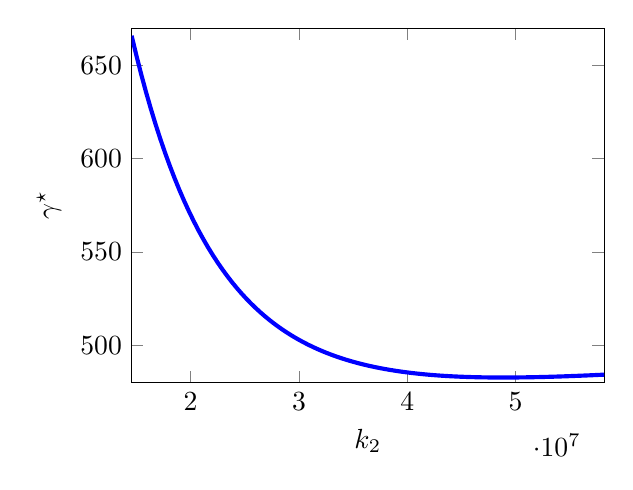
\begin{tikzpicture}

\begin{axis}[%
width=\fwidth,
height=\fheight,
scale only axis,
xmin=14546500, xmax=58186000,
ymin=480, ymax=670,
xlabel={$k_2$},
ylabel={$\gamma^{\star}$}]
\addplot [
color=blue,
solid,
line width=1.5pt,
forget plot
]
coordinates{
 (14546500,665.979118077888)(14987303.030303,655.36695313271)(15428106.0606061,645.360360576508)(15868909.0909091,635.924903476384)(16309712.1212121,627.028150672341)(16750515.1515152,618.639142554998)(17191318.1818182,610.728659022648)(17632121.2121212,603.269033180589)(18072924.2424242,596.234126859867)(18513727.2727273,589.599268935929)(18954530.3030303,583.341194208699)(19395333.3333333,577.437931672756)(19836136.3636364,571.868952207588)(20276939.3939394,566.614722461747)(20717742.4242424,561.657046980181)(21158545.4545455,556.978696809064)(21599348.4848485,552.563522887073)(22040151.5151515,548.396340651795)(22480954.5454545,544.462848464683)(22921757.5757576,540.749761517473)(23362560.6060606,537.244340037538)(23803363.6363636,533.934916209779)(24244166.6666667,530.810261821383)(24684969.6969697,527.859957334736)(25125772.7272727,525.074235497906)(25566575.7575758,522.443866733078)(26007378.7878788,519.960291868848)(26448181.8181818,517.615130319755)(26888984.8484848,515.40093442387)(27329787.8787879,513.310442421924)(27770590.9090909,511.336884113876)(28211393.9393939,509.47388649596)(28652196.969697,507.715471049418)(29093000,506.056001771724)(29533803.030303,504.49010816633)(29974606.0606061,503.012572990982)(30415409.0909091,501.619337460674)(30856212.1212121,500.305423835061)(31297015.1515152,499.066789993765)(31737818.1818182,497.899554120807)(32178621.2121212,496.799884453695)(32619424.2424242,495.763147035684)(33060227.2727273,494.789144414256)(33501030.3030303,493.872340130782)(33941833.3333333,493.008666674376)(34382636.3636364,492.198156565705)(34823439.3939394,491.437546779031)(35264242.4242424,490.722780600709)(35705045.4545455,490.052400507041)(36145848.4848485,489.424143638136)(36586651.5151515,488.835909445028)(37027454.5454545,488.285562038419)(37468257.5757576,487.771473114561)(37909060.6060606,487.291685009588)(38349863.6363636,486.844502384748)(38790666.6666667,486.428323288638)(39231469.6969697,486.041615510223)(39672272.7272727,485.682878882061)(40113075.7575758,485.350864469166)(40553878.7878788,485.044185788941)(40994681.8181818,484.76162123358)(41435484.8484848,484.501986241351)(41876287.8787879,484.264160870196)(42317090.9090909,484.04708698055)(42757893.9393939,483.849746652211)(43198696.969697,483.671208820638)(43639500,483.510536698244)(44080303.030303,483.366879386458)(44521106.0606061,483.239410679532)(44961909.0909091,483.127362511127)(45402712.1212121,483.02996928817)(45843515.1515152,482.946535095389)(46284318.1818182,482.875351156128)(46725121.2121212,482.817846524344)(47165924.2424242,482.771912126545)(47606727.2727273,482.738314166242)(48047530.3030303,482.715423479692)(48488333.3333333,482.702631865404)(48929136.3636364,482.699696623764)(49369939.3939394,482.706269753571)(49810742.4242424,482.721739565391)(50251545.4545455,482.745687027001)(50692348.4848485,482.777693339563)(51133151.5151515,482.817377719553)(51573954.5454545,482.864373281798)(52014757.5757576,482.918304817227)(52455560.6060606,482.978822831989)(52896363.6363636,483.045195062316)(53337166.6666667,483.117402456592)(53777969.6969697,483.19537704297)(54218772.7272727,483.280671947403)(54659575.7575758,483.369909067567)(55100378.7878788,483.463588147359)(55541181.8181818,483.560923388426)(55981984.8484849,483.663594010254)(56422787.8787879,483.770296916022)(56863590.9090909,483.881020679589)(57304393.9393939,483.995373714874)(57745196.969697,484.113228108596)(58186000,484.234351460531) 
};
\end{axis}
\end{tikzpicture}%
\caption{The optimal $\Htwo$ performance as a function of $k_2$.}
\label{fig:sampled}
\end{figure}

To assess the benefit of parametric programming for this example, we start by assuming a polynomial dependency of all the LMI variables on the parameter $\ppar$. See Table \ref{tab:degrees} for the selected polynomial degrees. We take $q = 2$. Subsequently, the application of Polya relaxations is compared to knot insertion, of which the results are given in Table \ref{tab:polya_insknot}. It is remarked that application of a Polya relaxation of degree $k$ yields the same increase in numerical complexity as the insertion of $k$ knots, which is confirmed by the computation times. In addition, note that both the upper bounds and the lower bounds resulting from knot insertion are tighter for all cases.

\begin{table}
	\centering
	\caption{Selected polynomial degrees of the LMI variables.} \vspace{0.2cm}
	\label{tab:degrees}
	\begin{tabular}{cc}
		\toprule
	  LMI variable & degree \\
	  \midrule
		$Q(\ppar),U(\ppar),V(\ppar)$ & $q$ \\
		$F(\ppar), L(\ppar)$ & $q+1$ \\
		\bottomrule
	\end{tabular}
\end{table}

\begin{table}
	\centering
	\caption{Polya vs. knot insertion for polynomial LMI variables with $q = 2$.} \vspace{0.2cm}
	\label{tab:polya_insknot}
	\begin{tabular}{cccccc}
		\toprule
	  degree Polya relaxation & 0     & 1     & 2     & 4     & 8     \\
	  primal objective        & 560.8 & 554.2 & 543.6 & 537.2 & 532.8 \\
	  computation time [sec]  & 2.12  & 0.80  & 0.98  & 1.05  & 1.44  \\
	  dual objective          & 445.9 & 451.4 & 462.4 & 468.6 & 472.3 \\
	  computation time [sec]  & 1.28  & 0.69  & 0.76  & 0.84  & 1.10  \\
	  \midrule
	  inserted knots          & 0     & 1     & 2     & 4     & 8     \\
	  primal objective        & 560.8 & 550.3 & 532.2 & 529.2 & 528.0 \\
	  computation time [sec]  & 0.77  & 0.82  & 0.87  & 1.05  & 1.46  \\
	  dual objective          & 445.9 & 467.8 & 472.0 & 474.8 & 475.8 \\
	  computation time [sec]  & 1.23  & 0.70  & 0.79  & 0.88  & 1.06  \\
		\bottomrule
	\end{tabular}
\end{table}

To reduce conservatism, a first possibility is to increase the polynomial degree of the LMI variables. Another option is to assume the LMI variables to be polynomial splines, which boils down to increasing the number of knots instead of the polynomial degree of these variables. A comparison is shown in Table \ref{tab:incdeg_knot}.

\begin{table}
	\centering
	\caption{Higher polynomial degree vs. more knots of LMI variables (no Polya relaxation or knot insertion)} \vspace{0.2cm}
	\label{tab:incdeg_knot}
	\begin{tabular}{cccccc}
		\toprule
	  Polynomial degree $q$ (0 knots) & 2     & 3     & 4     & 5     \\
	  primal objective                & 560.8 & 536.2 & 530.2 & 526.5 \\
	  computation time [sec]  	      & 2.24  & 0.95  & 0.94  & 1.00  \\
	  dual objective          	      & 445.9 & 481.1 & 495.4 & 501.0 \\
	  computation time [sec]  	      & 1.31  & 0.78  & 0.84  & 1.02  \\
	  \midrule
	  number of knots $(q = 2)$       & 0     & 1     & 2     & 3     \\
	  primal objective                & 560.8 & 532.0 & 522.6 & 518.4 \\
	  computation time [sec]          & 2.13  & 0.88  & 0.96  & 1.13  \\
	  dual objective                  & 445.9 & 487.2 & 497.7 & 503.5 \\
	  computation time [sec]          & 1.34  & 0.83  & 0.93  & 1.06  \\
		\bottomrule
	\end{tabular}
\end{table}


\subsection{(Convex) inner and outer approximations of nonconvex sets}
We consider the problem of approximating from the inside the feasible set $
\mathbf{P} \subset \R^n$ of a matrix inequality $P(\ppar) \succeq 0$. Two examples
from~\cite{Henrion_Lasserre_2012} concerning the approximation of the stability region of linear
systems are considered.

An inner approximation is easily determined by solving the parametric phase I feasibility
problem
\[
\begin{aligned}
\minimize_{x\in\R} &&& x \\
\subj              &&& P(\theta) + xI \succeq 0 \; .%
\end{aligned}
\]
The inner approximation to $\mathbf{P}$ is
\[
\mathbf{\hat{P}} = \{\ppar \in \R^n \, : x^\opt(\ppar) \geq 0 \}.
\]
From the solution of the dual problem
\[
\begin{aligned}
\minimize_{Y\in \S^m} &&& \Tr(YP) \\
\subj              &&& Y \succeq 0 \\
                   &&& \Tr(Y) = 1 \; ,%
\end{aligned}
\]
an outer approximation
\[
\mathbf{\bar{P}} = \{\ppar \in \R^n \, : \Tr(Y^\opt(\ppar) P(\ppar)) \leq 0 \}
\]
is found. Convexity of the inner (outer) approximations can be imposed by
constraining the Hessian of the objective functions to be positive (negative)
semidefinite.

Moreover, since there are no crossterms between $\ppar$ and the optimization
variables in the primal, we can derive a dual feasible point from its Lagrange
multipliers as described in Section~\ref{subsec:extensions}.

The first example considers the nonconvex polynomial matrix inequality
\[
\mathbf{P} = \{\ppar \in \R^2 \, : \, P(\ppar) = \begin{pmatrix} 1 - 16\ppar_1
\ppar_2 & \ppar_1 \\ \ppar_1 & 1 - \ppar_1^2 - \ppar_2^2 \end{pmatrix} \succeq
0 \}.
\]

Figure~\ref{fig:PMI1_Henrion2012} shows the nonconvex (left) and convex
(right) inner and outer approximations of the set $\mathbf{P}$, indicated in
dark gray. A degree 3 B-spline basis with 13 internal knots was chosen both
for the primal and the dual.

\begin{figure}
\centering
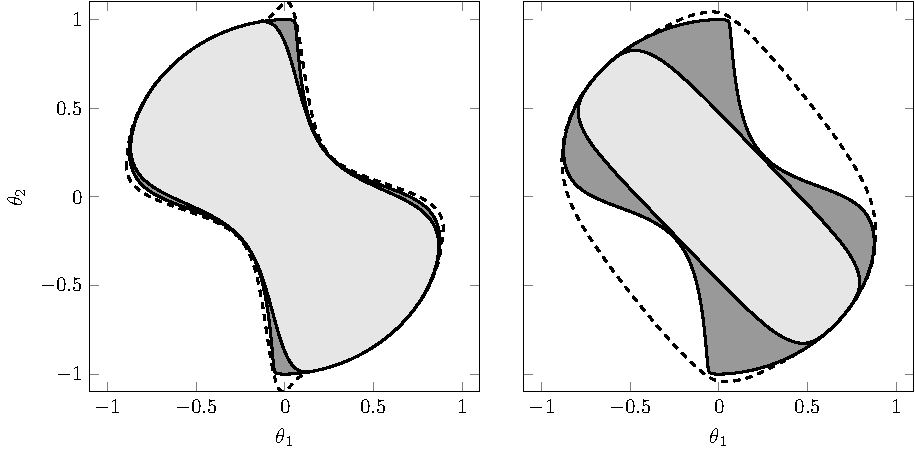
\includegraphics{figures/PMI1_Henrion2012_tikz.pdf}
\caption{Nonconvex (left) and convex (right) inner (solid) and outer (dashed)
approximations of the set $\mathbf{P}$}\label{fig:PMI1_Henrion2012}
\end{figure}

A second example considers the stability region of a degree 3 discrete-time
polynomial $z^3 + \ppar_1 z^2  + \ppar_2 z + \ppar_3$. The polynomial matrix
defining $\mathbf{P}$ is given by
\[
P(x) = \begin{pmatrix}
1 - \ppar_3^2 & \ppar_1 - \ppar_2 \ppar_3 & \ppar_2 - \ppar_1 \ppar_3 \\
\ppar_1 - \ppar_2 \ppar_3 & 1 + \ppar_1^2 - \ppar_2^2 - \ppar_3^2 & \ppar_1 -
\ppar_2 \ppar_3 \\
\ppar_2 - \ppar_1 \ppar_3 & \ppar_1 - \ppar_2 \ppar_3 & 1 - \ppar_3^2
\end{pmatrix}.
\]

\subsection{Approximate explicit model predictive control}
For linear systems, the classical MPC problem admits following parametric
formulation~\cite{Bemporad_et_al_2002}:
\[
\begin{aligned}
\minimize_{x \in \R^n} &&& \frac{1}{2} x^\t H x + \ppar^\t F x \\
\subj              &&& Gx \leq W + E\ppar \; ,
\end{aligned}
\]
where the parameters $\ppar$ denote the current state of the system and $x$
denotes the vector system inputs along the entire control horizon.

We consider Example 7.1 from~\cite{Bemporad_et_al_2002}. At first, we only
consider the constraint $-2 \leq x \leq 2$ without any state constraints such
that the optimization problem is feasible for all $\ppar$. Figure~ compares
the state and input trajectories of our approximate solution, parameterized by
a B-spline of degree 2 with 8 knots uniformly distributed over $[-1.5,
1.5]\times[-1.5, 1.5]$ \commentWVL{Perhaps we should speak of `mesh' instead
of `knots'?}, with those of the exact solution. Note that while there is
little loss in performance for the approximate solution, the evaluation of the
controller boils down to a simple function evaluation.

In case of state constraints, we follow the two step approach for infeasible
parameter values as discussed in Section~\ref{subsec:extensions}: by solving
the phase I problem we minimize the infeasibilities and subsequently we can
solve the optimization problem over $\Ppar$ by adding the minimal
infeasibility to the constraints. Note that even when the value of $\ppar$ is
infeasible for the original problem (e.g. due to disturbances), the
approximate solution still yields a control value.
Figure~\ref{fig:MPC_Bemporad2002} shows the state trajectory from an initial
condition $[-1, -0.8]$. The shaded area illustrates the feasible region for
the approximate parametric program.

\begin{figure}
\centering
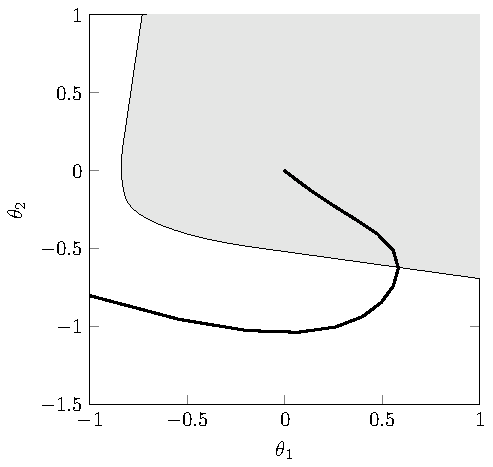
\includegraphics{figures/mpc_bemporad2002_if_tikz.pdf}
\caption{State trajectory for the approximate MPC starting from the infeasible
initial state $[-1, -0.8]$}\label{fig:MPC_Bemporad2002}
\end{figure}


\subsection{$\mathcal{H}_\infty$ optimization: solving BMI problems}
The $\mathcal{H}_\infty$ optimization problem of a static output feedback
controller on the linear system
\[
\begin{cases}
\dot{x} = Ax + B_1 w + Bu \\
z = C_1 x + D_{11} w + D_{12} u \\
y = Cx
\end{cases}
\]
can be cast as following parametric program
\[
\begin{aligned}
\minimize_{\gamma \in \R^+ \atop X \in \S^n} &&& \gamma  \\
\subj              &&&
\begin{pmatrix}
A_\pPar^\t X + X A_\pPar  &  XB_1  &  C_\pPar^\t \\
B_1^\t X                  & -\gamma I & D_{11}^\t \\
C_\pPar                   & D_{11}    & -\gamma I
\end{pmatrix} \preceq 0 \; ,
\end{aligned}
\]
where $A_\pPar = A + B \pPar C$ and $C_\pPar = C_1 + D_{12} \pPar C$ and $\pPar$
is the controller.

Assuming the parametric problem is feasible for all $\pPar \in \PPar \subset
\R ^{n_u \times n_y}$,\footnote {In case of infeasible parameter values, one
has to resort to finding the phase I problem for the constraint $A_\pPar^\t X
+ X A_\pPar \preceq 0, X \succeq 0$ as described in
Section~\ref{subsec:extensions}} the solution of the approximate parametric
optimization problem yields $\gamma (\pPar)$. Then, a simple box constrained
minimization of $\gamma(\theta)$ over $\PPar$ yields the optimal controller.
Note that the minimal value of the control polytope formed by the
coefficients of $\gamma$ and the mesh of Greville abscissae provides an
initial guess for the optimal controller.

The method is tested on data from the COMPl$_\text{e}$ib library
\commentWVL{ reference} and benchmarked with solutions from HIFOO
\commentWVL{reference}. As the problem size grows exponentially with the number of
parameters, the numerical examples are limited to a maximum 4 parameters. Table
... shows the value of $\gamma$ attained with HIFOO and the proposed method.
The results are very similar for both methods.



% \subsection{Case study: A multiparametric \textsc{lp} with polyhedral parameter set}
% Consider the following multiparametric \textsc{lp} reported in~\cite{Gal_1979} and subsequently treated
% in~\cite{Borrelli_et_al_2003}:
% \begin{gather*}
% \begin{aligned}
% \minimize_{x\in\R^2} &&& -2 x_1 - x_2\\
%              \subj   &&& x_1 + 3 x_2 \leq 9 - 2\ppar_1 +\ppar_2 \\%
%                      &&& 2 x_1 + x_2 \leq 8 + \ppar_1 - 2\ppar_2 \\%
%                      &&& x_1 \leq 4 + \ppar_1 + \ppar_2 \\%
%                      &&& x_1, x_2 \geq 0 \;,
% \end{aligned}
% \end{gather*}
% on $\Ppar \in [-10, 10] \times [-10, 10]$.

% It can be shown that for this problem $\Pfeas$ is a triangular set.
% Hence, the optimization variables cannot be parameterized by a tensor spline
% in $\theta_1$ and $\theta_2$ as this would render the problem infeasible.
% Instead, a parameterization is chosen that maps a rectangular domain to a
% polyhedral set.

% Consider a spline parameterization $(p_{\ppar_1}(\alpha),
% p_{\ppar_2}(\alpha))$ of the boundary of $\Pfeas$ in terms of a
% scalar parameter $\alpha \in [0, 1]$ \commentWVL{What about higher dimensions?
% Is it straightforward to parameterize such polyhedral sets?}. To `fill' the
% polydral set an additional variable $\beta \in [0, 1]$ is introduced. By
% defining $\ppar_1(\alpha,\beta) = p_{\ppar_1}(\alpha) \beta$ and
% $\ppar_2(\alpha,\beta) = p_{\ppar_2}(\alpha) \beta$, any $(\alpha, \beta)$ now
% maps to a feasible $\ppar_1, \ppar_2$. Similarly, $x$ can also be
% parameterized as a tensor spline in $\alpha$ and $\beta$.

% Figure~\ref{fig:mplp_objective} shows the approximated objective function for
% a tensor spline of degree 1. The accordance with the true objective function
% is good, except near the switch in critical regions, as shown in
% figure~\ref{fig:mplp_error}.

% \begin{figure}
% \centering
% 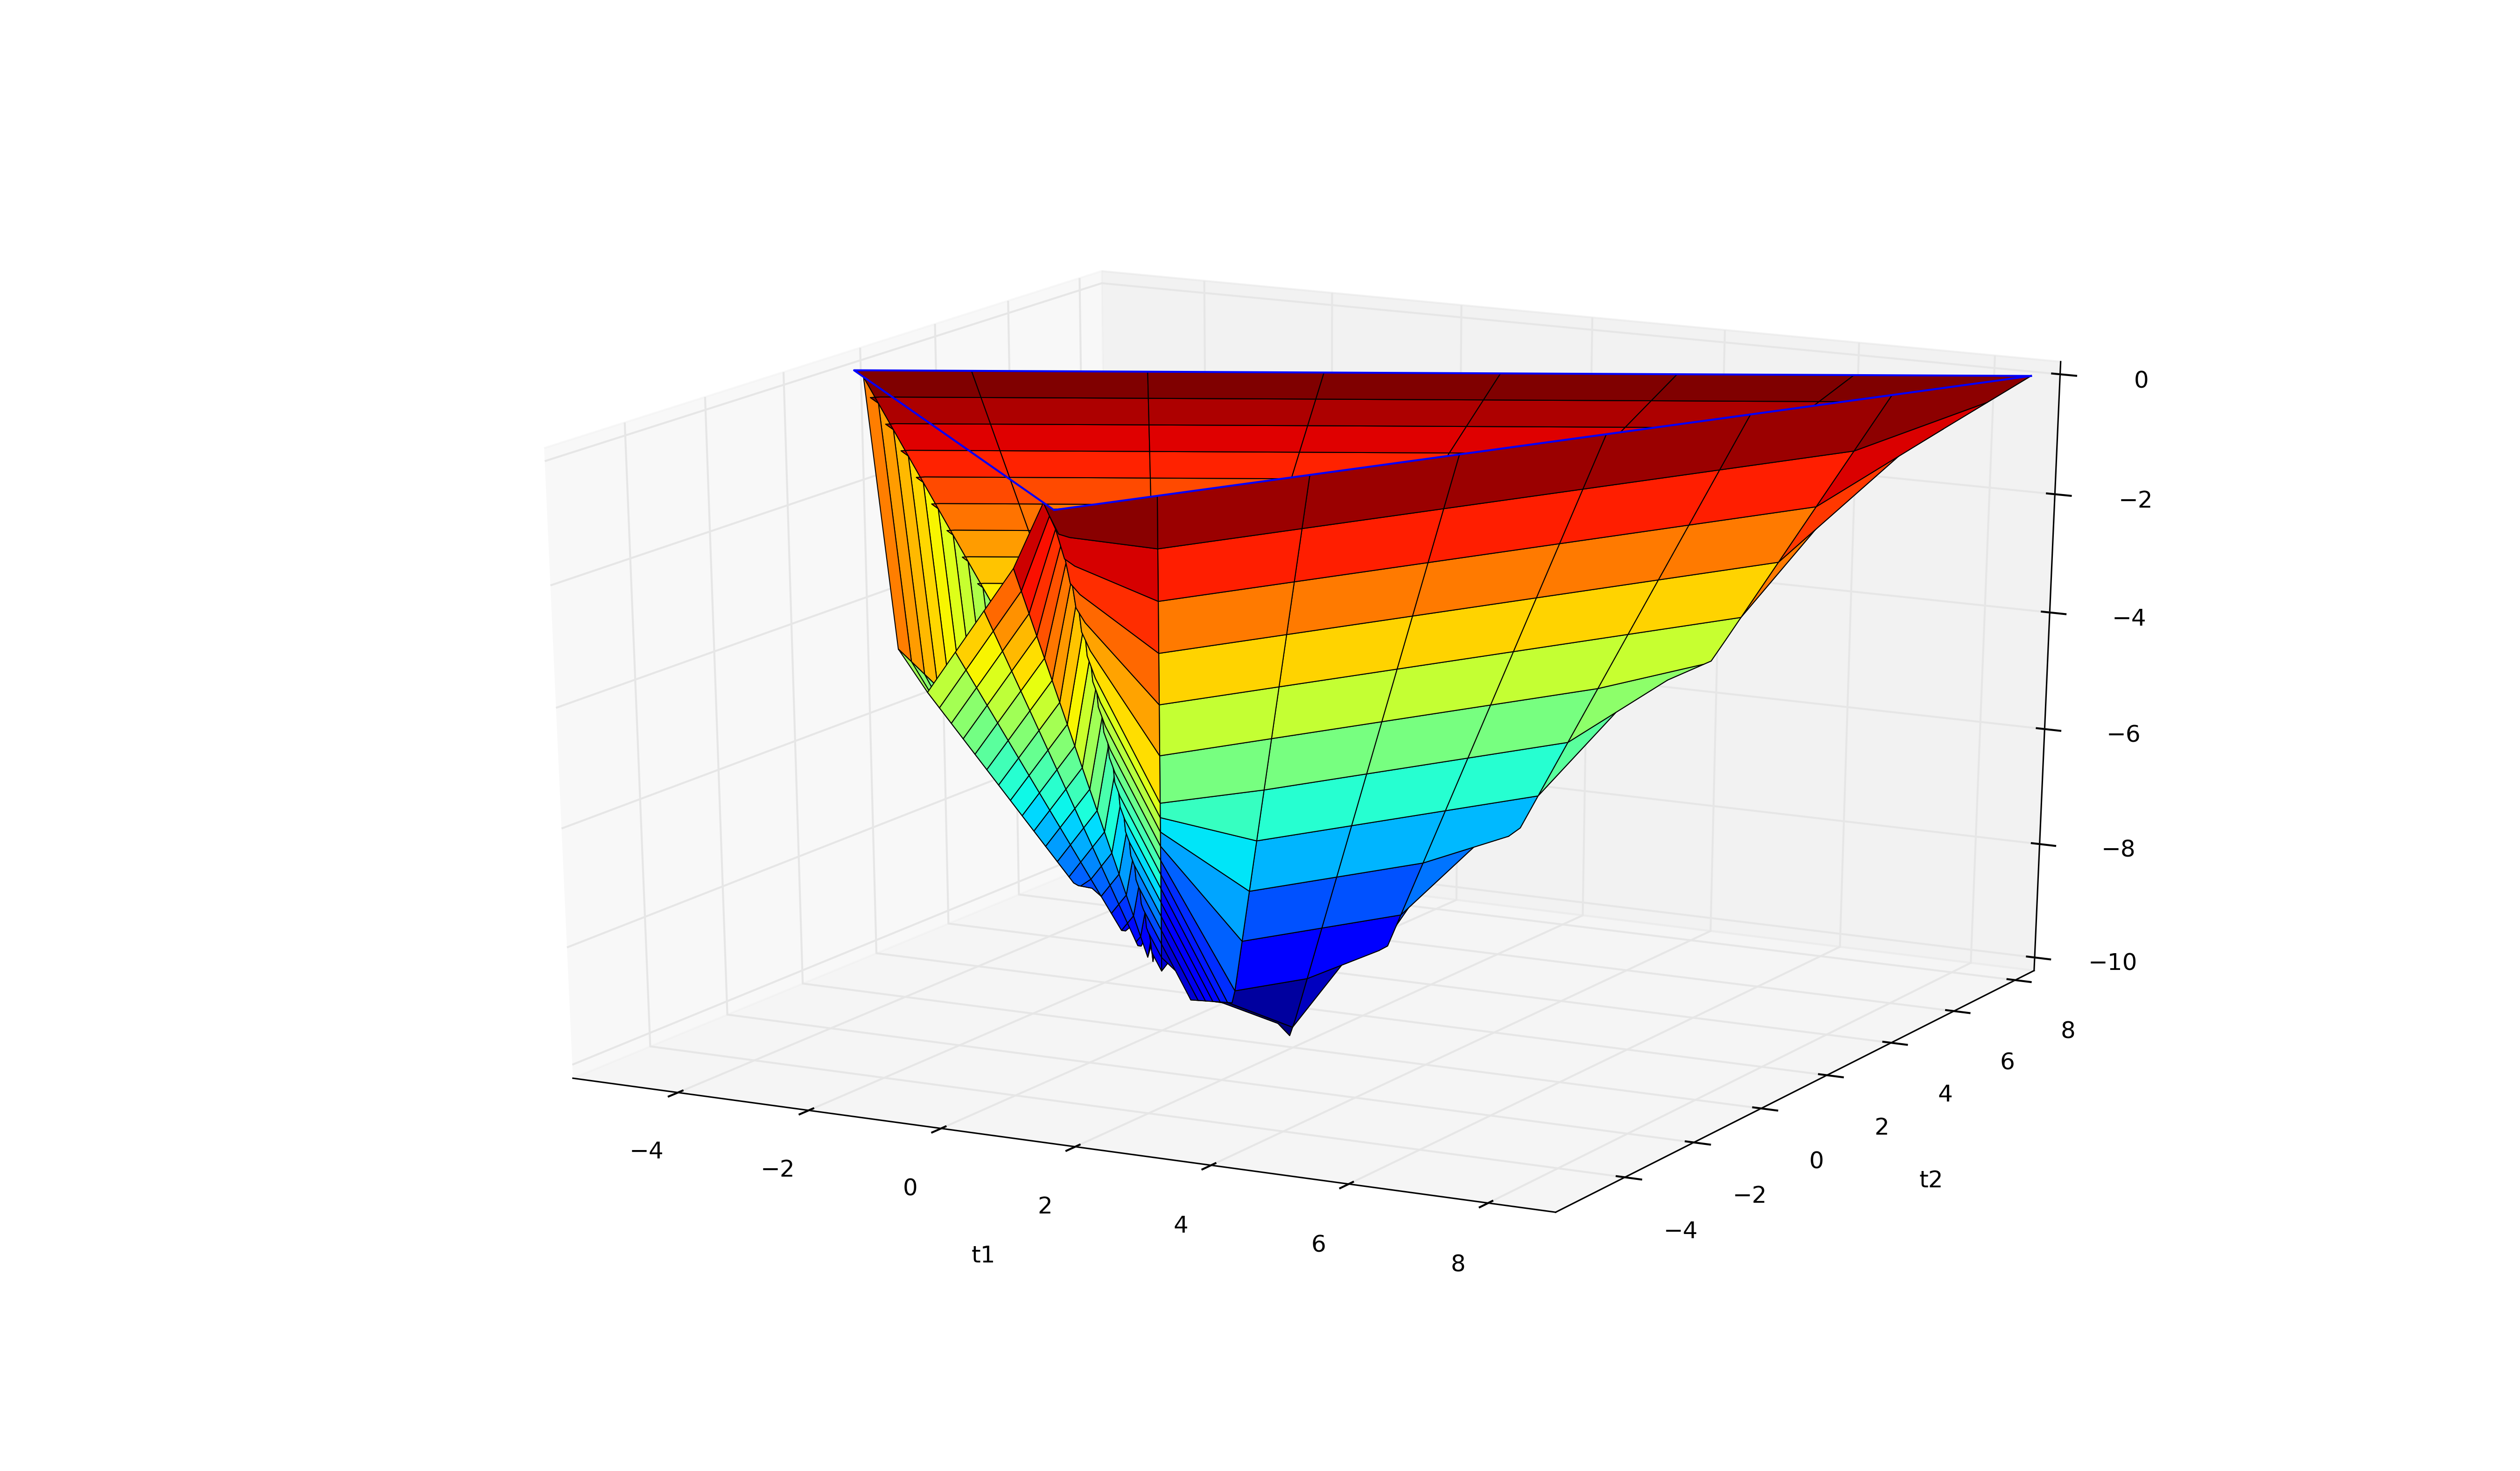
\includegraphics[width=0.8\textwidth]{figures/mplp_poly_objective.png}
% \caption{The approximated objective function for a degree 1 tensor product
% spline with 21 equidistantly spaced knots in $\alpha$ and 51 in $\beta$.}
% \label{fig:mplp_objective}
% \end{figure}

% \begin{figure}
% \centering
% 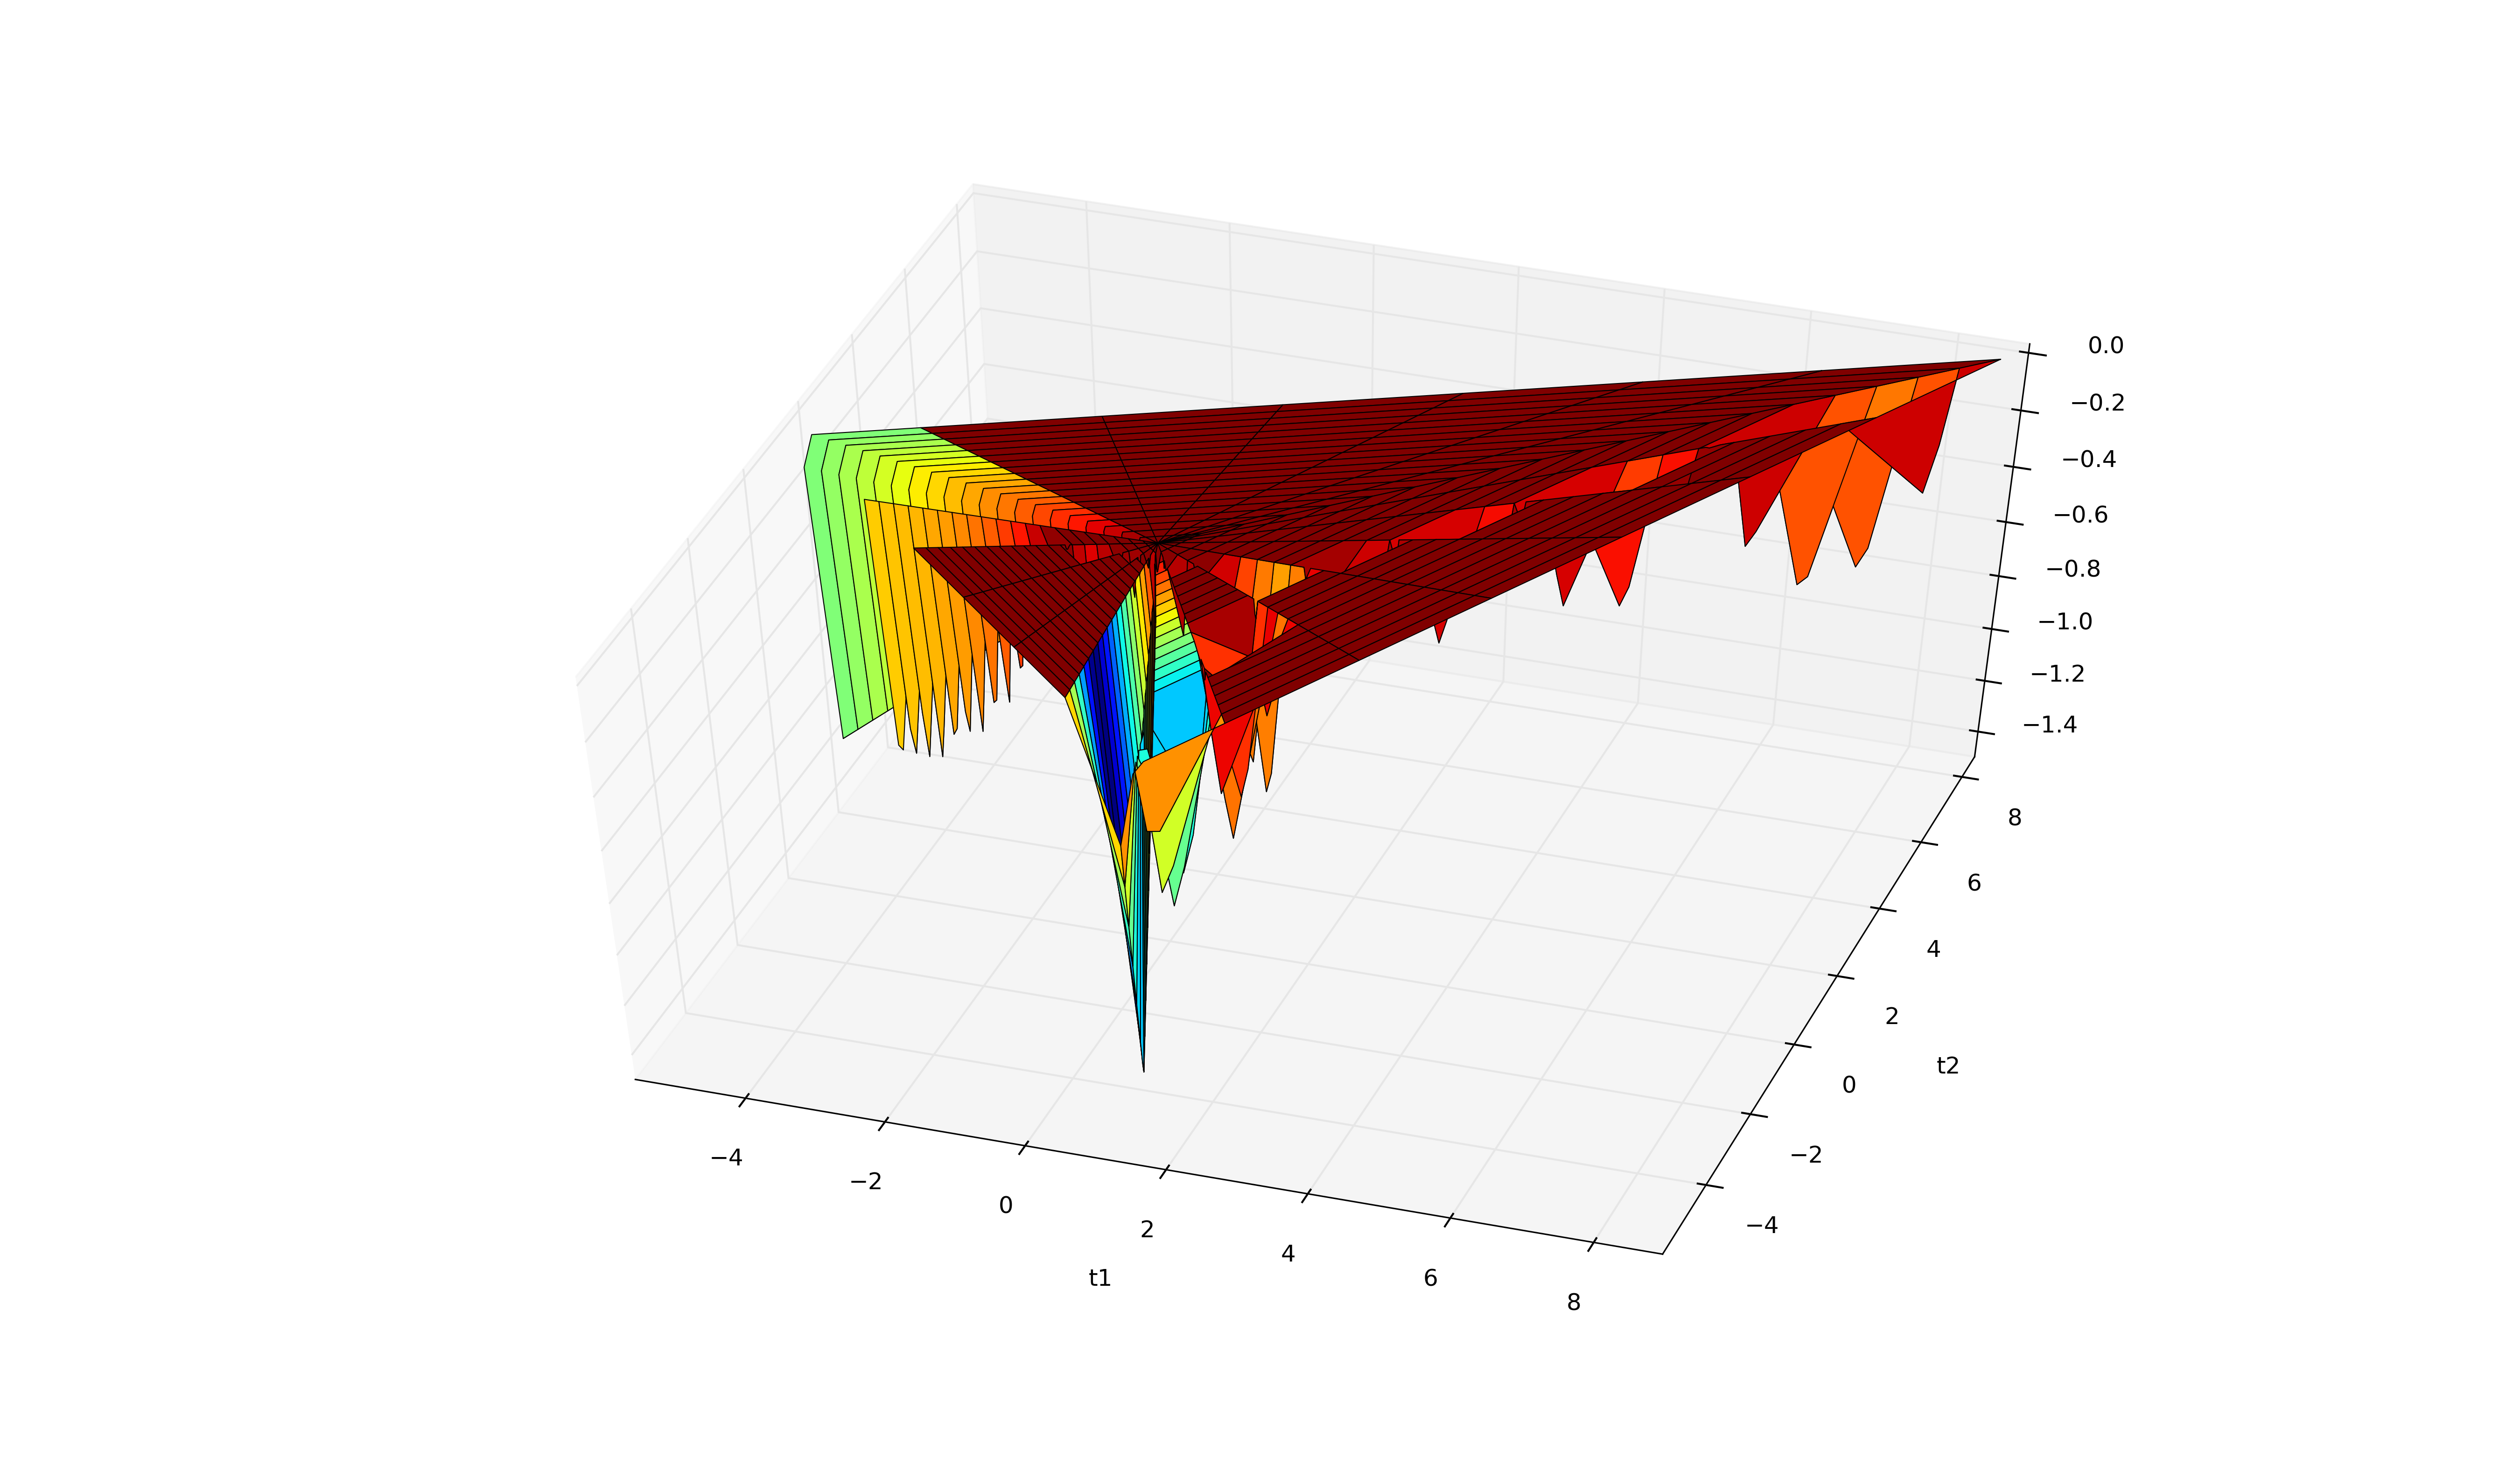
\includegraphics[width=0.8\textwidth]{figures/mplp_poly_error.png}
% \caption{The error between the true value of the objective function and our
% approximation.}
% \label{fig:mplp_error}
% \end{figure}

%%%%%%%%%%%%%%%%%%%%%%%%%%%%%%%%%%%%%%%%%%%%%%%%%%%%%%%%%%%%%%%%%%%%%%%%%%%%%%
%%%%%%%%%%%%%%%%%%%%%%%%%%%%%%%%%%%%%%%%%%%%%%%%%%%%%%%%%%%%%%%%%%%%%%%%%%%%%%

\appendix
\section{Sums and products of B-splines}

\[
    \xi = (\xi_1, \ldots, \xi_l)
\]
and the $i$-th normalized B-spline function of degree $k$, defined on $[\xi_i, \xi_{i+k+1})$, is computed using the Cox-de Boor recursive formula
\commentWVL{add reference}:
\[
    b_{i,k,\xi}(x) = \frac{x-\xi_i}{\xi_{i+k} - \xi_i}
    b_{i,k-1,\xi}(x) +
    \frac{\xi_{i+k+1}-x}{\xi_{i+k+1} - \xi_{i+1}}
    b_{i+1,k-1,\xi}(x) ,
\]
starting with
\[
    b_{i,0,\xi}(x)  =
    \begin{cases}
        1 , \text{if } x \in [\xi_i , \xi_{i+1} ) , \\
        0, \text{if } x \notin [\xi_i , \xi_{i+1} ) .
    \end{cases}
\]

Sums and products of splines with bases $b_{k,\kappa}$ and $b_{l,\lambda}$ with
can be expressed in a new basis $b_{m, \mu}$.

For a sum of two splines, we find
\[\mu_i = \]

\bibliographystyle{plain}
\bibliography{references/pprog}


\end{document}
